\begin{figure}[h]
    \centering

    \begin{subfigure}[b]{0.45\textwidth}
        \centering
        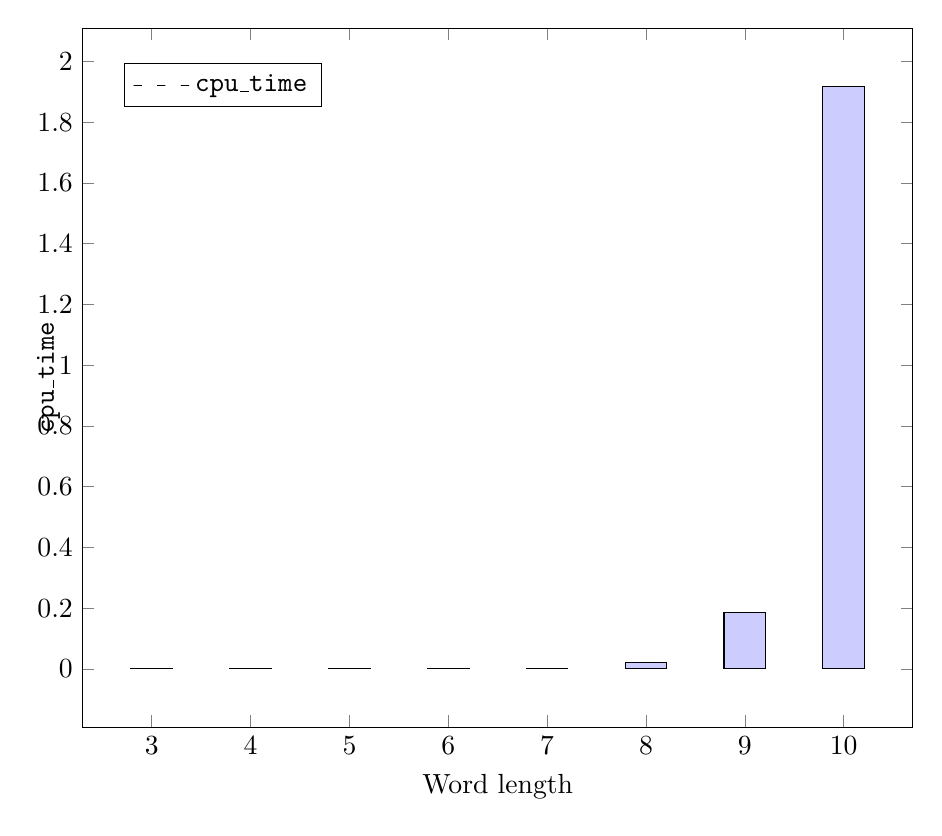
\begin{tikzpicture}
            \begin{axis}[
                xlabel=Word length,
                ylabel=\texttt{cpu\_time},
                ylabel style={yshift=-15pt},
                xtick=data,
                width=\linewidth,
                legend style={at={(0.05,0.95)},anchor=north west},
                ]
            \addplot[ybar, bar width=15pt, fill=blue!20]
                coordinates {
                    (3, 9.238719940185547e-06)(4, 2.132143293108259e-05)(5, 8.704112126277044e-05)(6, 0.0004073193198756168)(7, 0.0026500152267572535)(8, 0.020409859716892242)(9, 0.18663626367395575)(10, 1.9177763095268836)
                    };
            \legend{ \texttt{cpu\_time} } 
            \end{axis}
        \end{tikzpicture}
    \end{subfigure}
    % \hfill
    \begin{subfigure}[b]{0.45\textwidth}
        \centering
        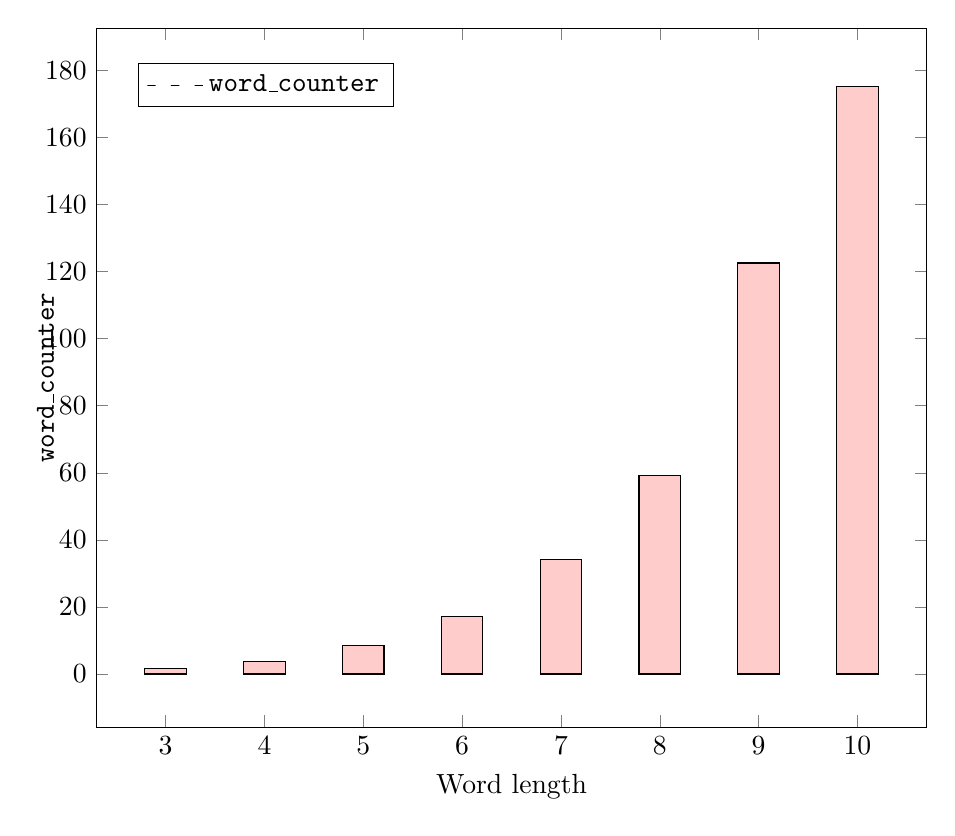
\begin{tikzpicture}
            \begin{axis}[
                xlabel=Word length,
                width=\linewidth,
                ylabel=\texttt{word\_counter},
                ylabel style={yshift=-10pt},
                xtick=data,
                legend style={at={(0.05,0.95)},anchor=north west}
                ]
            \addplot[ybar, bar width=15pt, fill=red!20]
                coordinates {
                    (3, 1.5)(4, 3.619047619047619)(5, 8.576923076923077)(6, 17.263157894736842)(7, 34.25190839694657)(8, 59.0625)(9, 122.5909090909091)(10, 175.23076923076923)
                    };
            \legend{ \texttt{word\_counter} } 
            \end{axis}
        \end{tikzpicture}
    \end{subfigure}
    \caption{Performances testing through process}
\end{figure}